In this section, we describe the interface with which a user can interact with our retrieval system.
Figure \ref{fig:gui-overview-app} shows the window that is opened to the user when the application is launched.
The user can select a folder with 3D shapes (the system will show only the files that have the extension \verb!".ply"!),
as shown in Figure \ref{fig:gui-overview-file-browser}.
To retrieve similar shapes, the user selects what shape they want to query on, and after clicking, a preview 
of the 3D shape is opened.
After closing the preview window, a query is performed when the \textbf{Retrieve similar shapes} button is selected.
The system returns a list of shapes according to the query, and a preview of 1--5 retrieved shapes is displayed.
The user also has the ability to use the system for retrieving all the shapes within a distance range in both default
and advanced modes.

If the query shape is present in our database, the system will find it internally with a distance of 0 - since it
is most similar to itself.
We don't consider this to be desirable for an end user, so the query shape is not returned as part of the results.
After closing the preview, the user can see the retrieved shapes' filenames, as well as the distance between each 
retrieved shape and the query.
Clicking on a shape from the retrieved list opens a 3D preview window with that shape. 

By default, the system uses a pre-computed index on the features database.
This index is constructed with a technique called Approximate Nearest Neighbours (ANN), which is discussed in detail 
in Section \ref{section:scalability}.
\begin{figure}[H]
    \centering
    \begin{subfigure}[b]{0.45\textwidth} 
        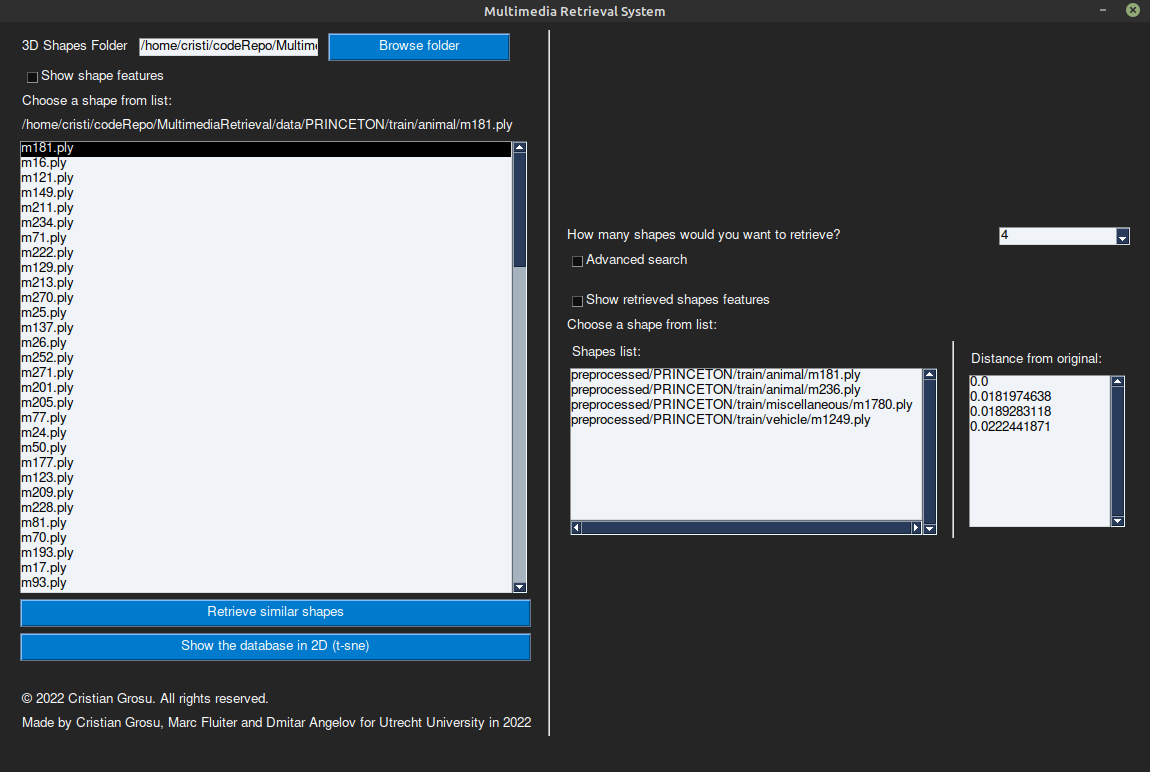
\includegraphics[width = \textwidth]{assets/GUI/retrieval_ann_example.png}
        \caption{System overview}
        \label{fig:gui-overview-app}
    \end{subfigure}
    \hfill
    \begin{subfigure}[b]{0.45\textwidth} 
        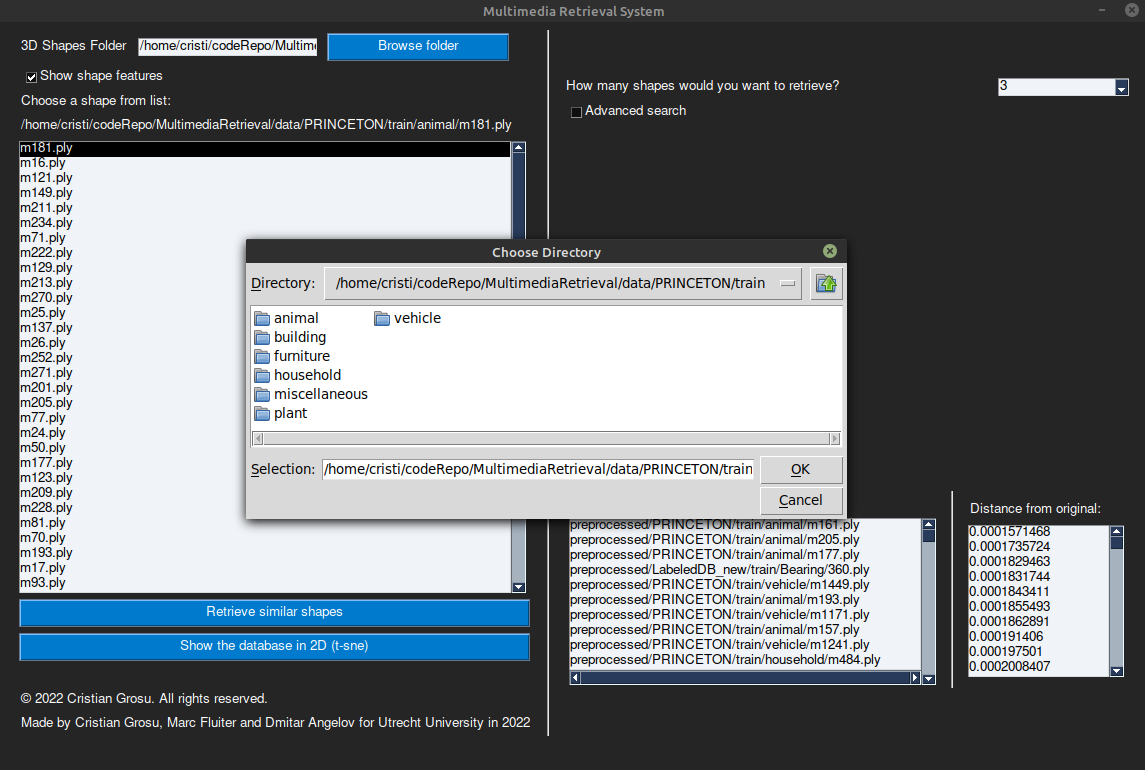
\includegraphics[width = \textwidth]{assets/GUI/folder_browser.png}
        \caption{Browsing shapes folders}
        \label{fig:gui-overview-file-browser}
    \end{subfigure}
    
    \caption{Multimedia retrieval system overview}
    \label{fig:gui-overview}
\end{figure}

\subsection{Advanced mode}
Optionally, the user can enter an advanced query mode by checking the\textbf{Advanced search} checkbox.
This allows the user to tune the distance functions, change the weights of certain features, and more.
Figure \ref{fig:gui-advanced-knn} shows the options which are available to the user when in advanced mode.

A set of new fields are displayed, in which the user can indicate how to weigh different parts of the feature
vector and which distance function they would prefer to use.
By default, the scalar distance function is the cosine distance, and the distance function for the histograms is the
Earth Mover's Distance (EMD).
The scalar distance functions are weighted in a 3:1 ratio to the histogram distance function.

\begin{figure}[H]
    \centering
    \begin{subfigure}[b]{0.45\textwidth} 
        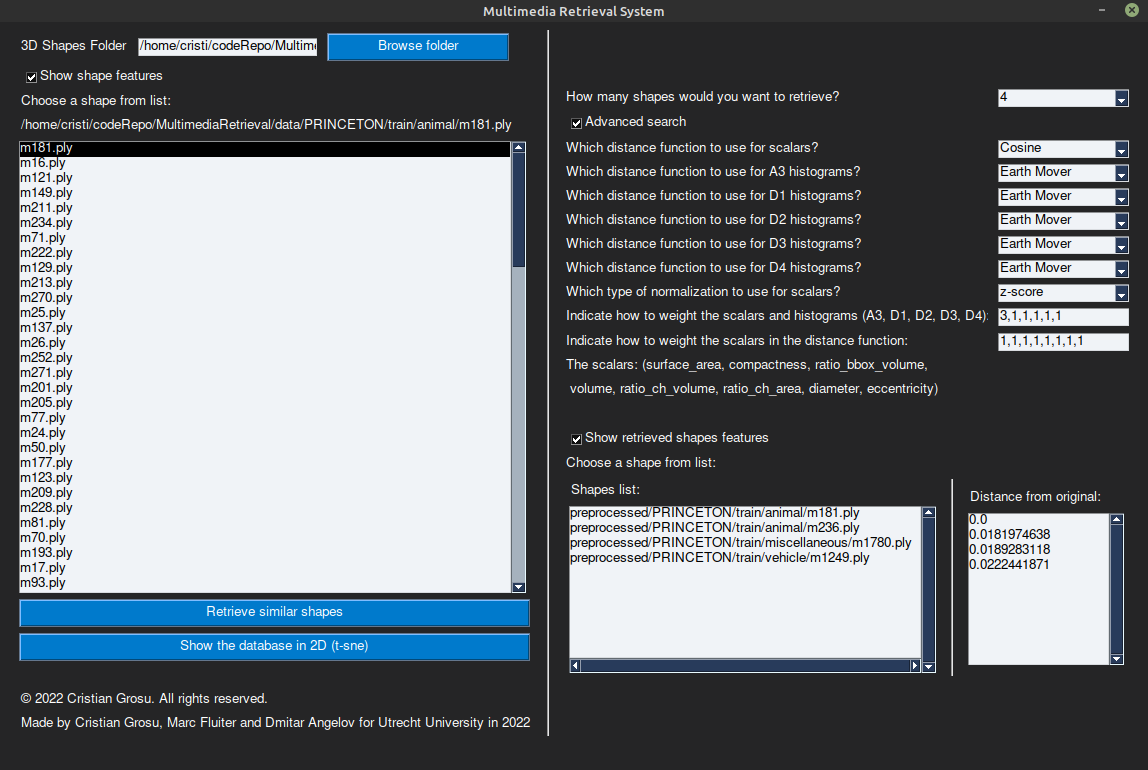
\includegraphics[width = \textwidth]{assets/GUI/retrieval_knn_example.png}
        \caption{Advanced retrieval indicating $k$}
        \label{fig:gui-advanced-knn}
    \end{subfigure}
    \hfill
    \begin{subfigure}[b]{0.45\textwidth} 
        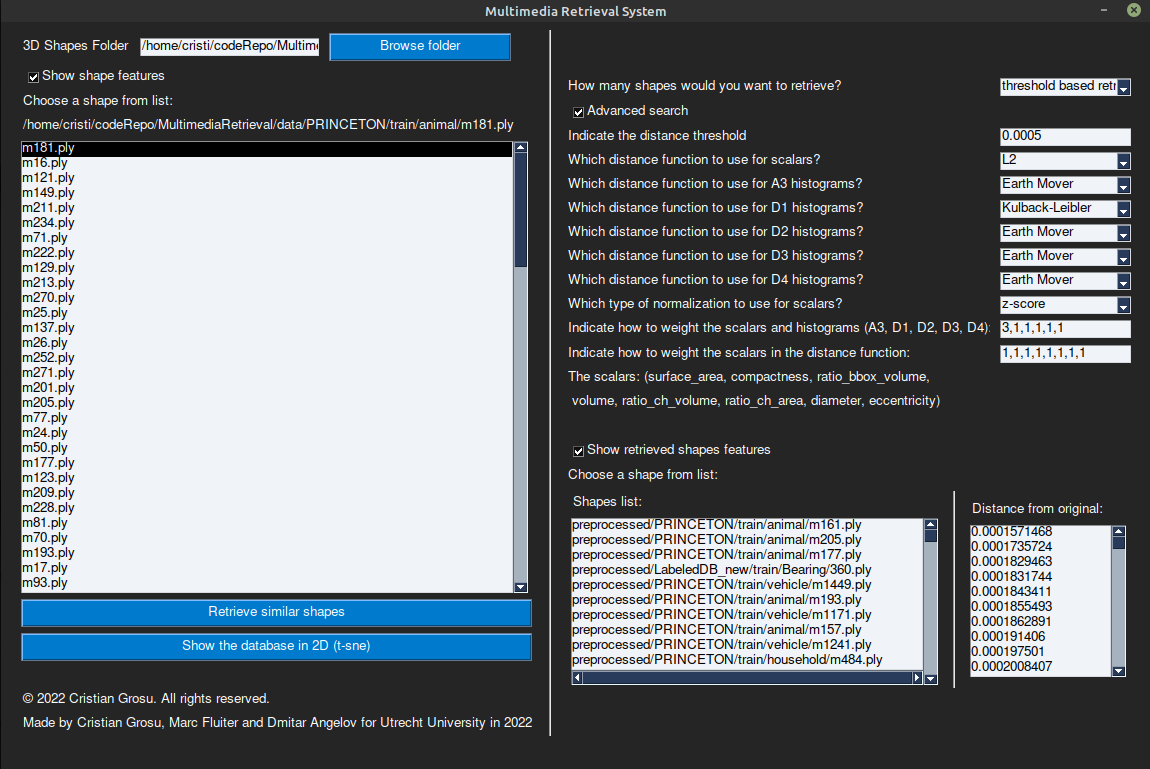
\includegraphics[width = \textwidth]{assets/GUI/retrieval_threshold_based.png}
        \caption{Advanced threshold-based retrieval}
        \label{fig:gui-advanced-threshold-based}
    \end{subfigure}
    \hfill
    
    \caption{Advanced retrieval}
    \label{fig:gui-advanced}
\end{figure}